\textcite{vlaanderen_staat_2019} estimated there were around 71.000 cases of Campylobacteriosis in the Netherlands in 2018, 67.000 in 2017 and 79.000 in 2016. We plotted the amount of cases produced by our model against the average of these three values. The results can be seen in Figure~\ref{fig:val_human_cases}. Our 

\textcite{nepluvi_rapportage_2019} monstered broiler chickens weekly in 2018, and found $41,9$-$58.1\%$ of broilerchickens were tested positive for \textit{Campylobacter}. This concerns chickens from slaughterhouses. As can be seen in Figure~\ref{fig:val_chickens}, our base model has similar values for each year.

In the Netherlands the (unsanitary) preparation and/or consumption of chicken were attributed to $20$-$30\%$ of infections in 2018. However, around $50$-$80\%$ of cases can be attributed to \textit{Campylobacter} strains associated with poultry \parencite{cuperus_surveillance_2020, nepluvi_rapportage_2019}. Therefore, it is safe to assume that there are multiple transmission routes. We assume the biggest transmission routes can be found in the environment. In the base model, around 5.70\% of the infections stem from the preparation and/or consumption of chicken. This can be seen in Figure~\ref{fig:val_sources}. It may be the case that the environment plays a bigger role than we previously assumed, after all, it is easier to trace back the cause to undercooked meat than to a wild bird.

We also validated our DALYs and Cost of Illness against the datapoints from \parencite{mangen_campylobacteriosis_2007}. Note that these values are from 2007. As can be seen in Figure~\ref{fig:val_dalys} our model determines higher DALYs than given in the literature. This may indicate that there are more chronic diseases that can be traced back to \textit{Campylobacter} than is currently happening in the real world. Perhaps the specialists are overlooking the bacterium as a cause, or they are simply unable to pinpoint the cause.

In Figure~\ref{fig:val_coi} it can be seen that the Cost of Illness calculated by the model is lower than \citeauthor{mangen_campylobacteriosis_2007}'s values. This is probably due to the fact that we only look at 3 chronic conditions and the acute conditions. 

It is estimated there are around 17 million species of \textit{Diptera} per person \parencite{gorman_trillions_2017}. We are only interested in \textit{Musca domestica}. It is unknown what their numbers are in the Netherlands, and we are unable to estimate. However, it has been guessed that the population of Houseflies will increase by 244\% by 2080 \parencite{mcalister_secret_2017}. In The amount of flies in our model after 1 year is 20.000 of which 7.700 are infectious (TIME STEP = 0.0625). This is probably not a proper reflection of the real world, but one can assume that it is only 7.700 flies that have directly caused a disease in humans and/or chickens.

The model also includes an Infection risk from birds (2.5e-05). There are about 1.3 million birds in the Netherlands \parencite{noauthor_miljoenen_2019}. There was no literature on the risk from birds, so we assumed a somewhat safe value. We doubt \textit{Campylobacter} will ever be exterminated due to the presence of these environmental factors, even if we are somehow able to keep our farms, slaughterhouses and stores free from \textit{Campylobacter}.

%to include: meat consumption

\begin{figure*}[!h]
    \centering
    \begin{minipage}{0.45\textwidth}
        \centering
        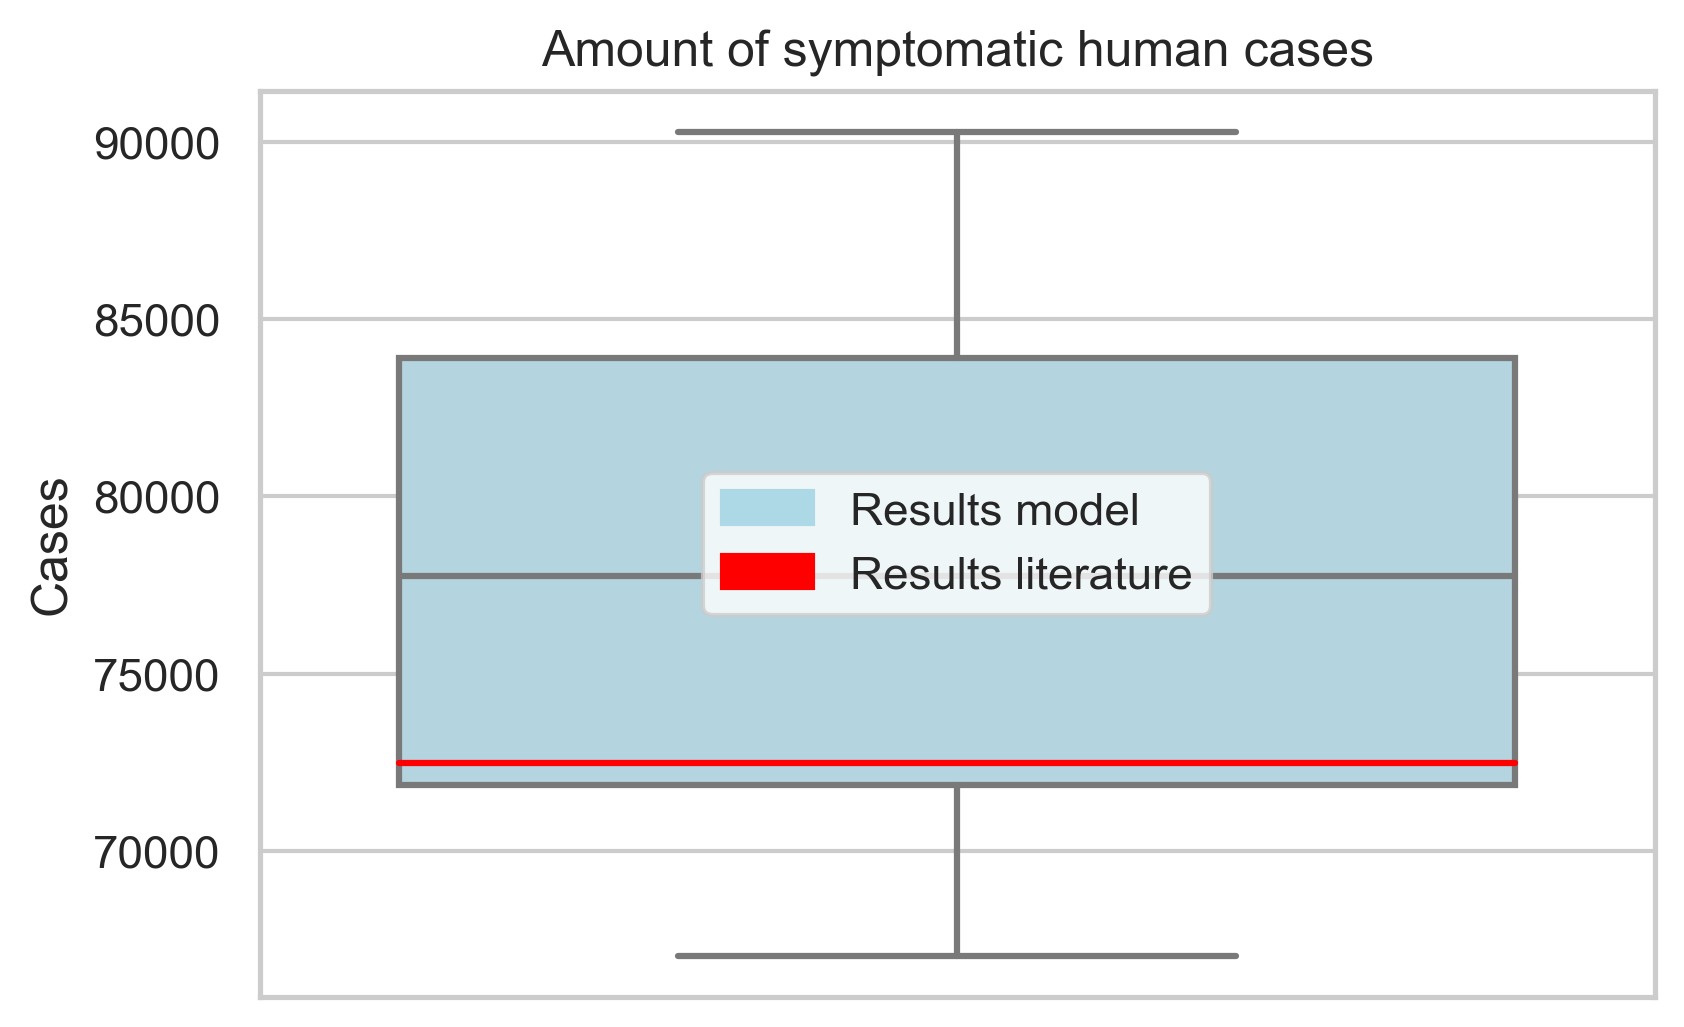
\includegraphics[width=0.9\textwidth]{notebooks/human_cases2.png} % first figure itself
        \caption{Validation of human cases}
        \label{fig:val_human_cases}
    \end{minipage}\hfill
    \begin{minipage}{0.45\textwidth}
        \centering
        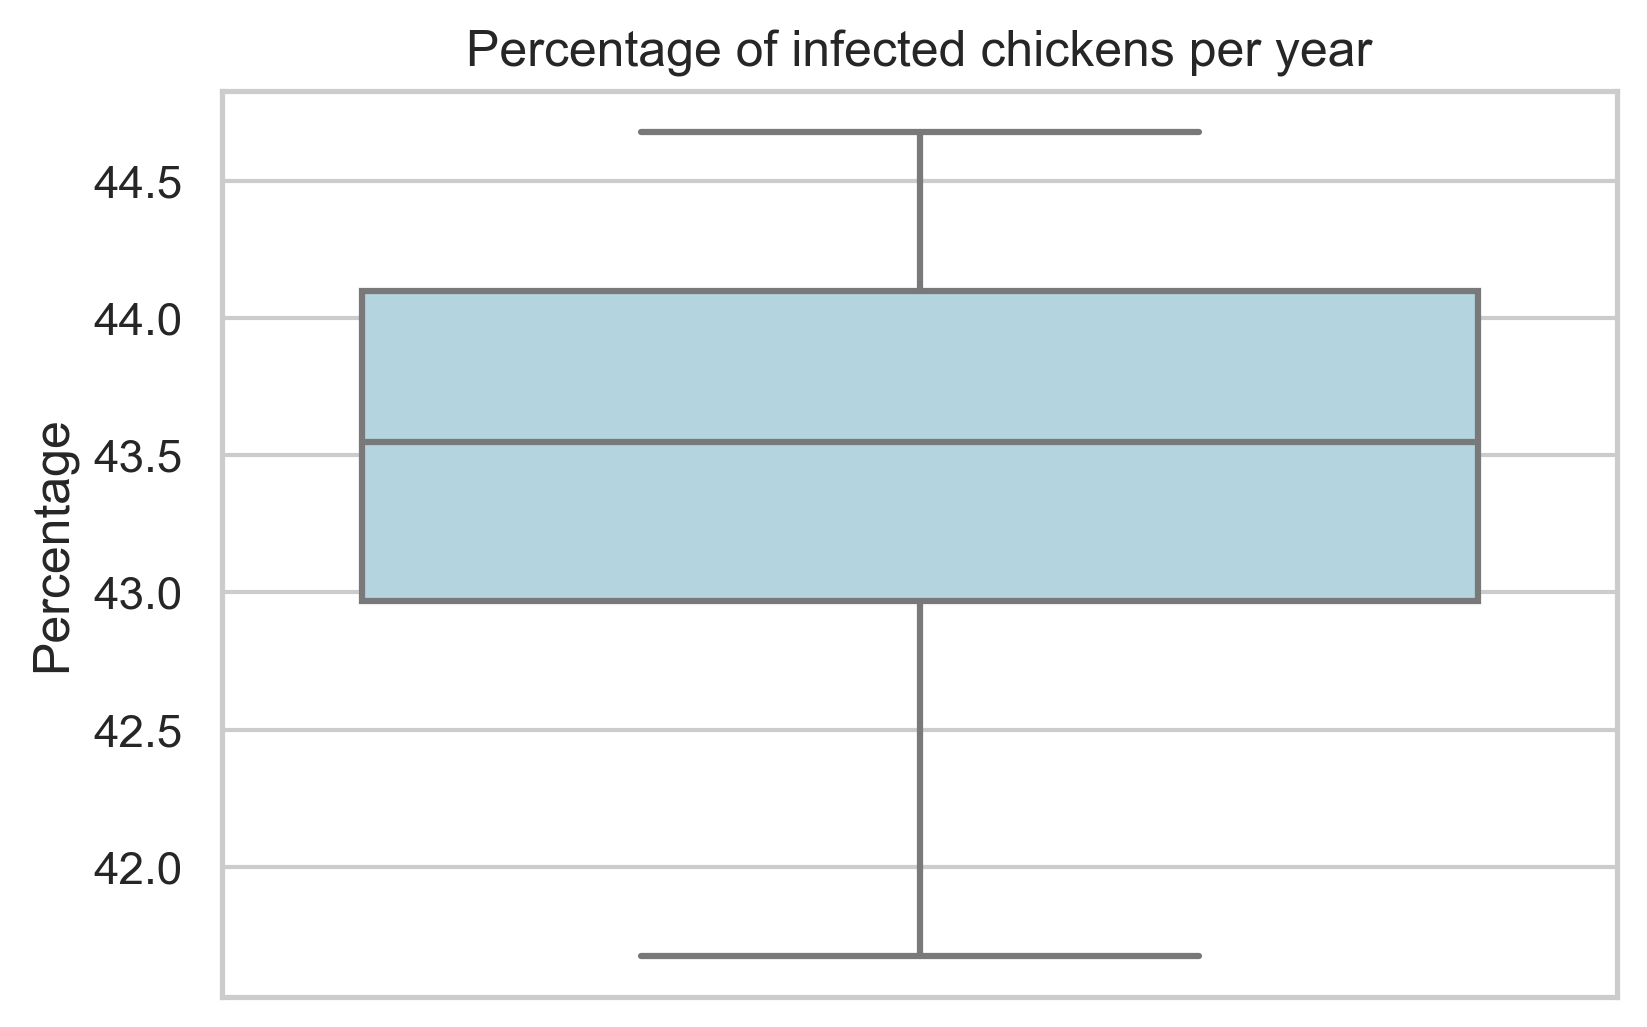
\includegraphics[width=0.9\textwidth]{notebooks/chickens2.png} % second figure itself
        \caption{Validation of proportion infected chickens}
	    \label{fig:val_chickens}
    \end{minipage}
\end{figure*}

\begin{figure*}[!h]
	\centering
	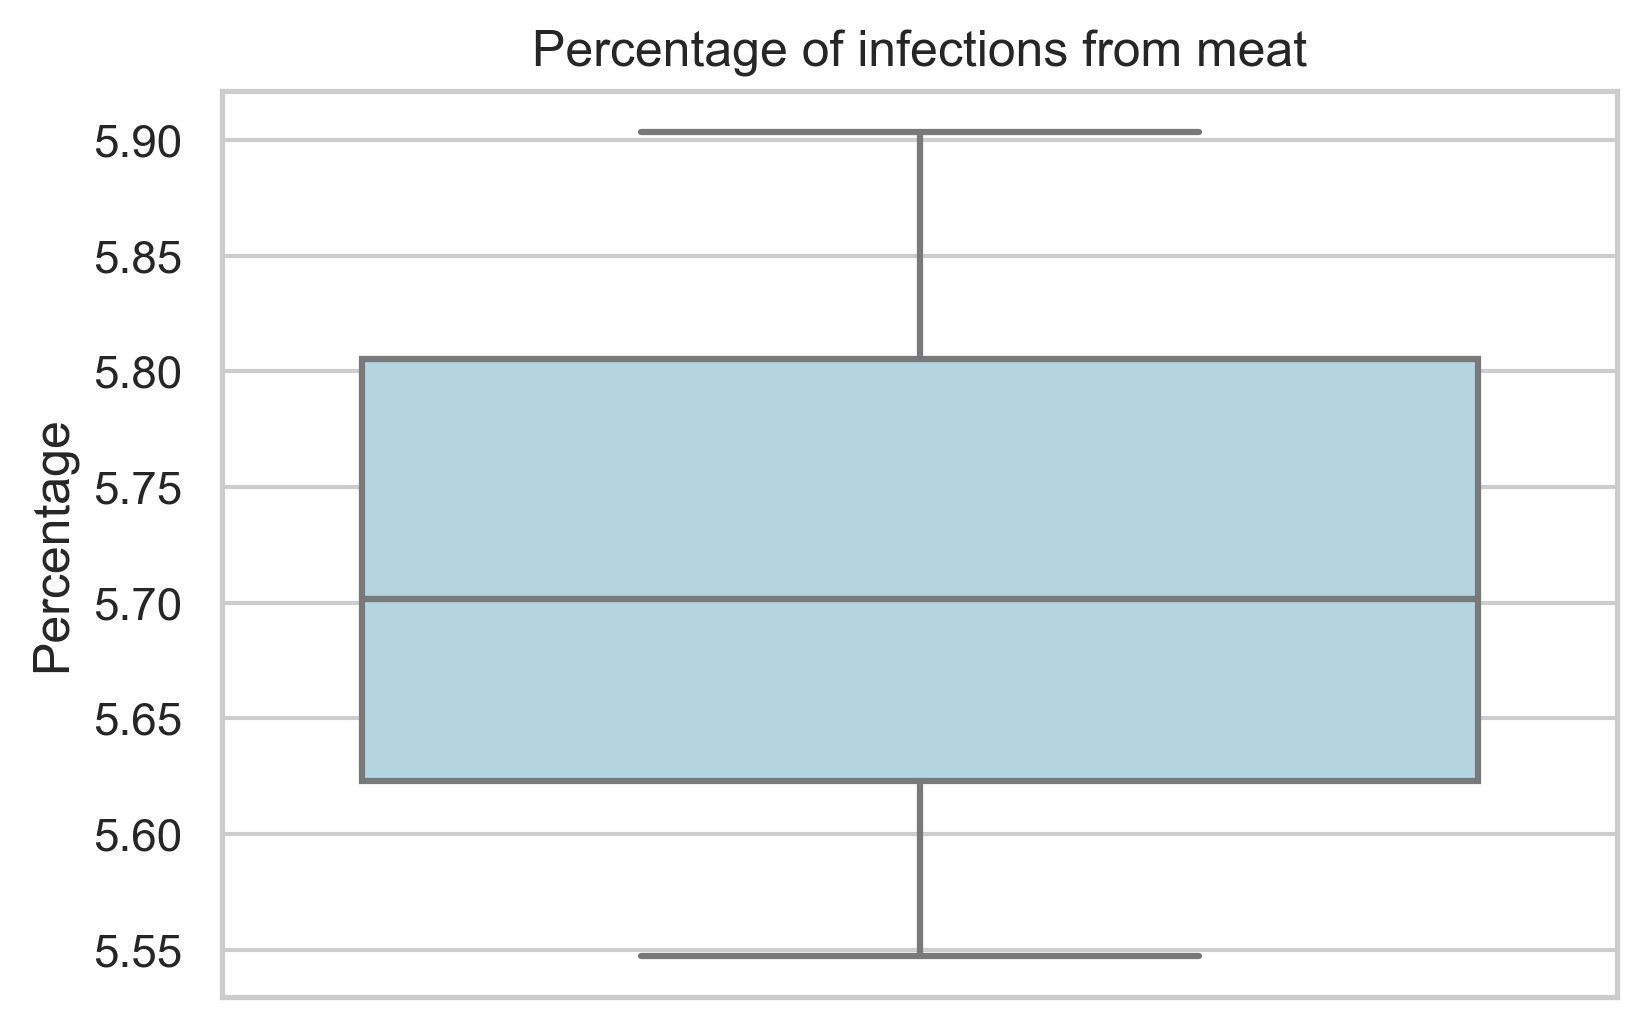
\includegraphics[width=0.5\textwidth]{notebooks/source2.png}
	\caption{Validation of sources of Campylobacteriosis}
	\label{fig:val_sources}
\end{figure*}

\begin{figure*}[!h]
    \centering
    \begin{minipage}{0.45\textwidth}
        \centering
        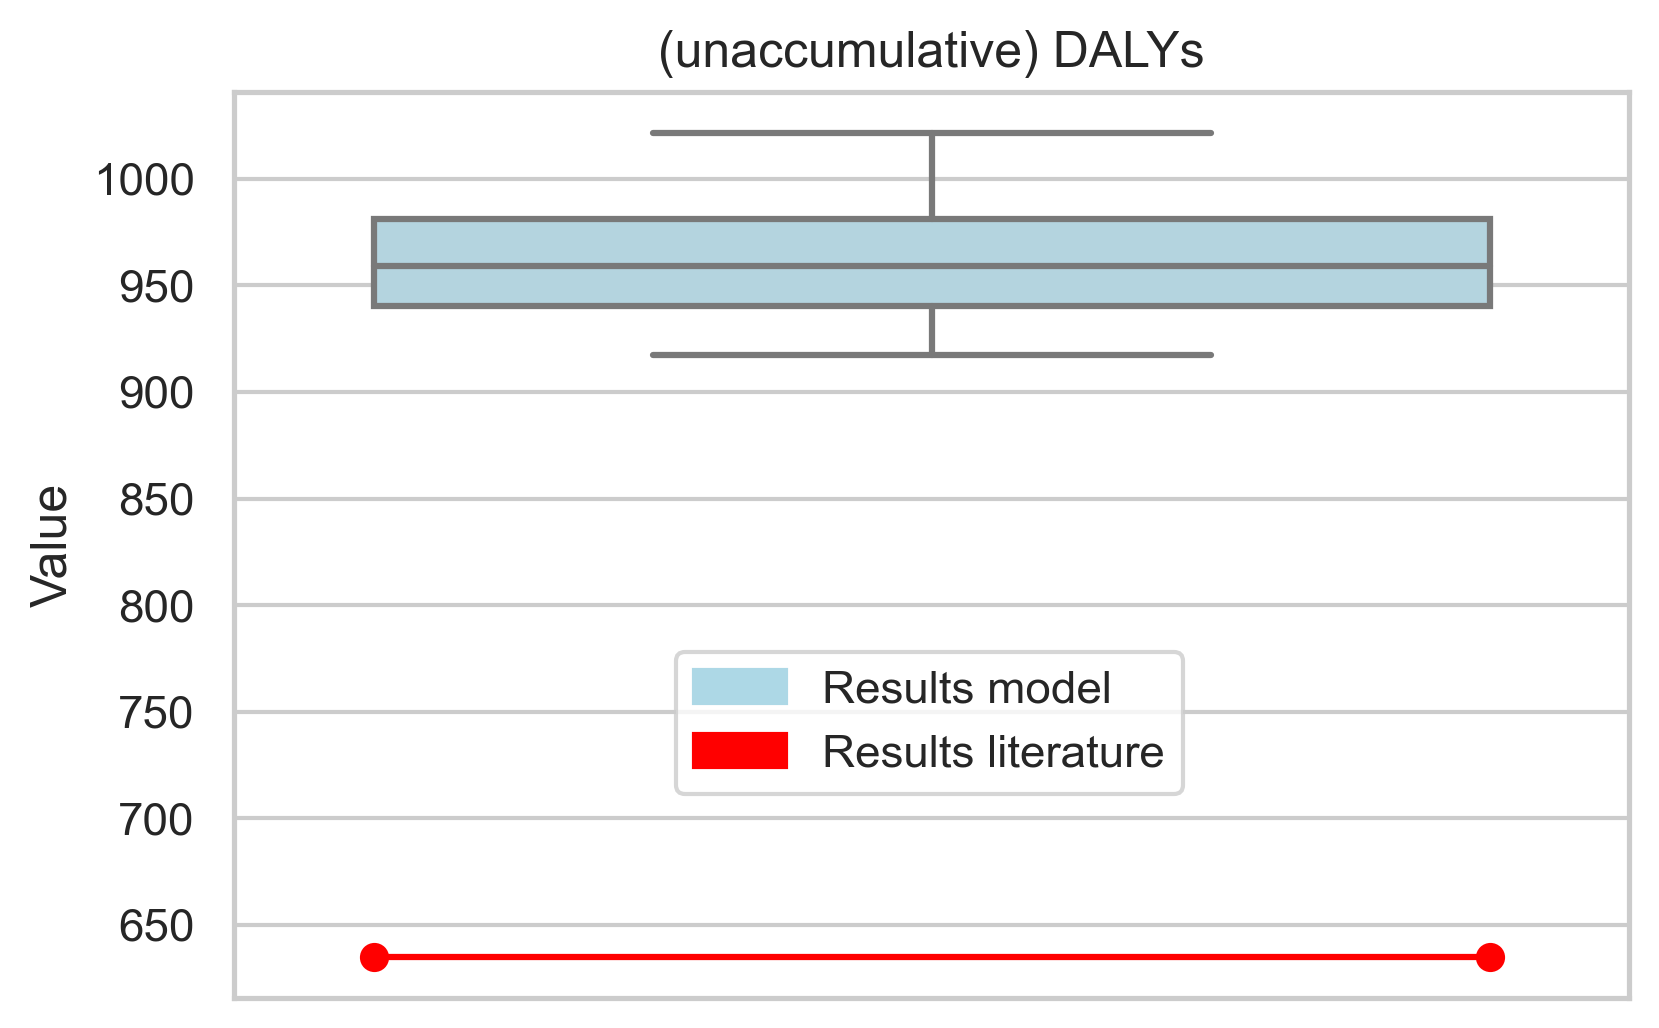
\includegraphics[width=0.9\textwidth]{notebooks/dalys2.png} % first figure itself
        \caption{Validation of DALYs}
	    \label{fig:val_dalys}
    \end{minipage}\hfill
    \begin{minipage}{0.45\textwidth}
        \centering
        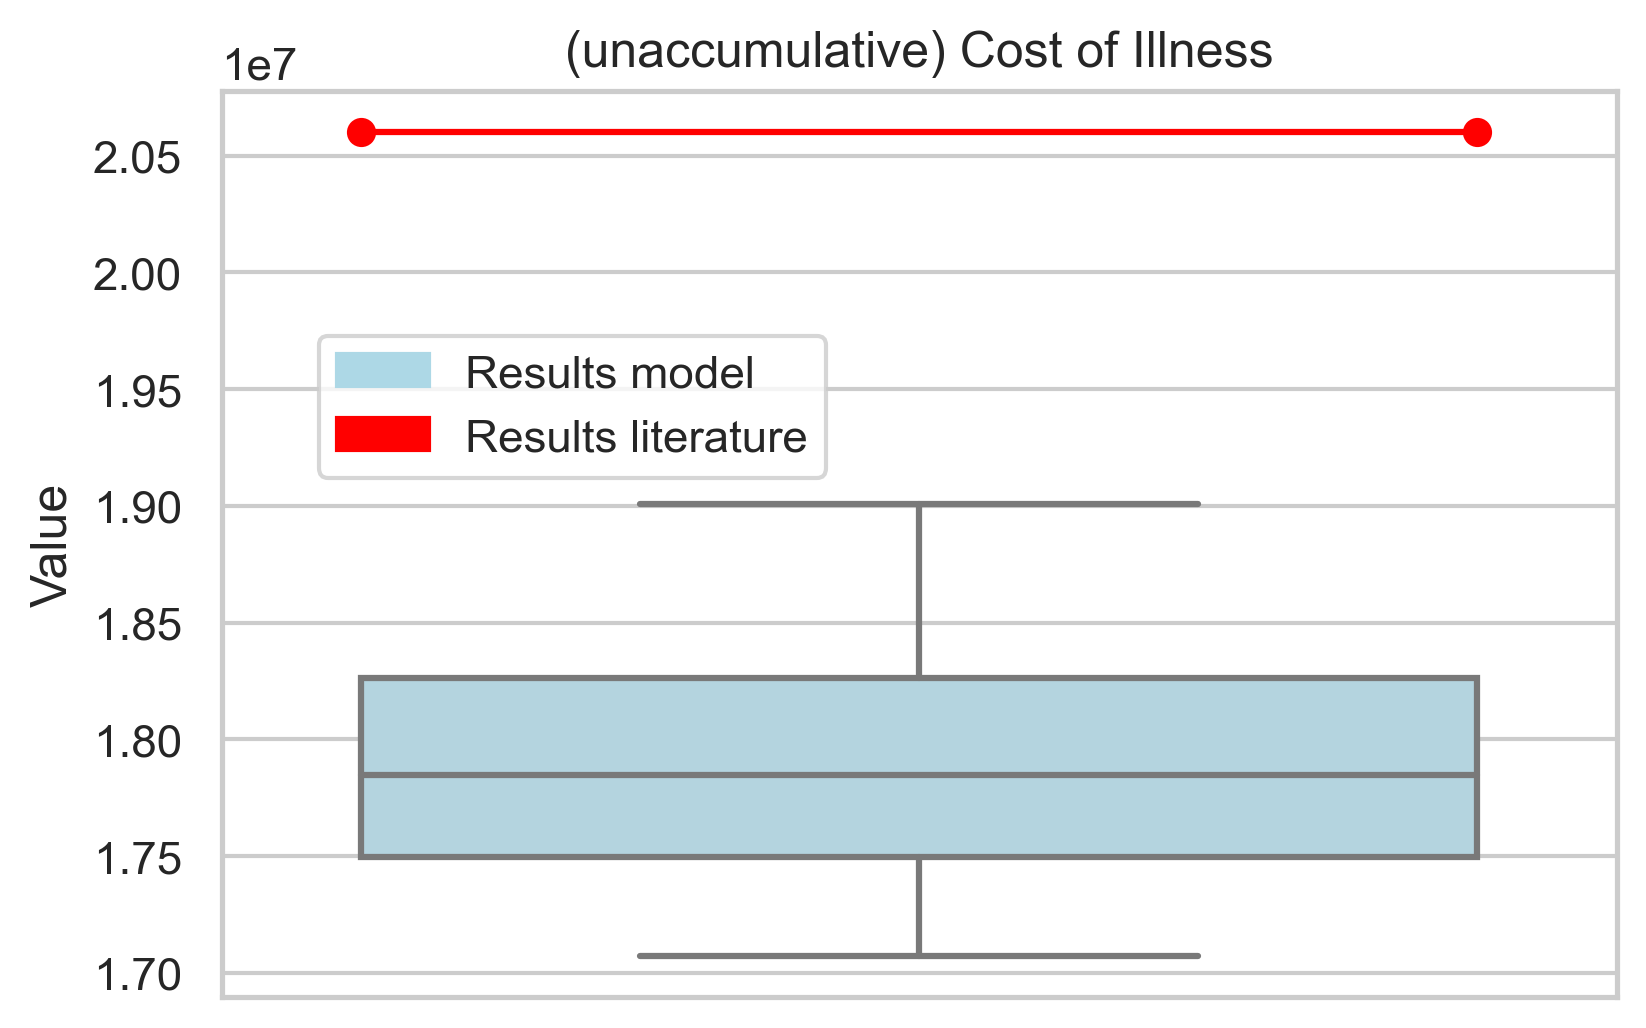
\includegraphics[width=0.9\textwidth]{notebooks/coi2.png} % second figure itself
        \caption{Validation of Cost of Illness}
	    \label{fig:val_coi}
    \end{minipage}
\end{figure*}